\documentclass{article}
\usepackage[utf8]{inputenc}
\usepackage{graphicx}
\usepackage{enumitem}
\usepackage{array}
\graphicspath{ {images/} }

\title{Physics 111A- Lab 1\\
Introductory Experiments and Linear Circuits I}
\author{Joshua Levy }
\date{August 2016}

\begin{document}

\section{Prelab}

\paragraph{Part 1} ~\\

\begin{enumerate}
    \item Write a short paragraph each explaining how the breadboard, power supply, multimeter, oscilloscope, and the signal/pulse generator are used. 
    \begin{itemize}
        \item Breadboard- Breadboards are used to create temporary circuits that do not require soldering. They house circuitry and make connecting various parts of the circuit very easy. These breadboards are useful for quick rearrangements and prototyping circuits. It is an insulating board with a series of holes to be used as sockets. As you plug in circuitry into the sockets, these elements are connected to each other by the wiring underneath that follow a certain pattern.
        \item Power Supply- There are two power supplies built into the box carrying the breadboard. The bottom terminal supplies 5V and is used with digital currents. There is also a 12V supply for the circuit. The ground can be attached to the 0V terminal. It supplies power to the breadboard.
        \item Multimeter- Multimeters can be separated into two categories, DVM (Digital Volt Meter, digital) and VOM (Volt Ohm Meter, analog). Both types of multimeters can make various measurements of different parts of circuits, including voltage, current and resistance. The analog meter uses a magnet to deflect a pointer attached to a wire carrying current, thereby allowing you to make the reading that you would see on an analog scale. At its core, the DVM senses voltage across a tiny resistor and can infer resistance and current. The multimeter has a display, selection knob, and ports. The display will output the amount and item of measurement to a screen or pointer system. You can use the selection knob to select what you are measuring and the scale that you choose to measure it at. Hook up probes to the relevant ports; some ports allow you to measure larger currents. Place the two probes on each end of the circuit element you wish to measure. https://learn.sparkfun.com/tutorials/how-to-use-a-multimeter
        \item Oscilloscope- The oscilloscope is used to show how signals (detailing voltage, current, etc.) change over time. Essentially they can measure voltage differences and other features of the circuit and generate neat graphical displays for our measurement. The oscilloscope has four basic controls – the “vertical system, horizontal system and trigger system”, and the vertical position knob, which affect display outputs. The vertical system control changes the divisions marking the voltages on the displays, allowing you to resize signals of different amplitudes. The vertical position knob moves the output of the scope up or down. The horizontal system control changes divisions marking time on the horizontal axis of the display so you can change the scaling of time. The trigger button allows you to “stabilize” a repeated signal or check out an individual pulse. In order to get a measurement, you need to input a signal from your circuit to the input terminal. (xyz oscilloscope)
        \item Signal/Pulse Generator- The lab uses a function generator, which outputs various voltage signals to the circuit, allowing you to make sine, triangle and square waves over a large range of frequencies. To see these signals, connect the output cable of this generator to the input of the oscilloscope (or to the circuit) and turn the channel on/off button on. To output a particular waveform, press one of the waveform buttons below the screen. You can change the attributes of the wave by pressing the back button until a menu pops up giving you options. 
    \end{itemize}
    \item What is the difference between the common and the ground of a circuit? \\
    The ground of a circuit is any lead, wire, or bus somehow connected to the earth, and we usually set this reference point to be 0V of potential. Grounding a piece of equipment seriously reduces the chance of getting shocked or electrocuted. However, it is not necessary to “ground” equipment. You can define a reference point that is not connected to the earth, that all other measurements of the circuit are made with respect to. You can set this reference point to be 0V. We’ll call this the “common”. All grounds are commons but not all commons are grounds.
    \item Derive the voltage divider equation (VoutVin=R2R2+R1) for the following circuit: ... see figure in lab handout \\
    \begin{equation}
        I_{short} = \frac{V_{in}}{R_1 + R_2} 
    \end{equation}
    \begin{equation}
        I_{short} = \frac{V_{out}}{R_2} 
    \end{equation}
    Setting (1) and (2) equal through substitution...
    \begin{equation}
        \frac{V_{in}}{R_1 + R_2} = \frac{V_{out}}{R_2}
    \end{equation}
    Multiplying both sides by $\frac{R_2}{V_{in}}$ achieves:
    \begin{equation}
        \frac{V_{out}}{V_{in}} = \frac{R_2}{R_1 + R_2}
    \end{equation}

\end{enumerate}


\paragraph{Part 2}

\begin{enumerate}
    \item What is impedance? Input impedance? Output impedance?
    \begin{itemize}
        \item Impedance, $Z$, is the new quantity used to describe complex resistance when $V$ and $I$ are not in phase. Resistance is the real part of impedance while reactance $X$ is the imaginary part, $Z = R + jX$, where $j$ is a substitute for imaginary $i$. The equation for impedance is still $V = Z*I$, but now $V$ and $I$ are out of phase and are time varying. To find instantaneous impedance, take $\frac{dV}{dI}$ or approximate it with $\frac{\delta V}{\delta I}$. Essentially, impedance is the measure of the opposition of current flow, but takes into account dynamic processes. It may be a function of frequency.
        \item Input impedance is the Thévenin’s equivalent impedance $Z_{in} = \frac{V_{open}}{I_{short}}$ , the ratio of the open-circuit voltage to the short-circuit current, and is the measure of the opposition of current flow in both static (resistance, eg. resistors) and dynamic (reactance, eg. capacitors and inductors) from the source voltage to the load. 
        \item Output impedance is very similar to the input impedance but is used in different scope. Whereas input impedance is found through measuring an input signal, output impedance is found by finding the Thévenin’s equivalent impedance of a signal device’s output terminals.

    \end{itemize}
    \item What are the interesting properties of a coaxial cable and transmission lines? (hint: Wikipedia.org)
    \begin{itemize}
        \item Coaxial cables- Coaxial cables conducts electrical signals using an inner conductor, which is surrounded by a dielectric insulating layer, enclosed by a metallic shield typically held at ground potential, finally enclosed by an insulating jacket. The dielectric layer and the metallic shield keep electric and magnetic fields from leaking and outside fields are kept from interfering with internal signals; thus, these cables can better transmit weak signals without interference. There is less leakage from cables with larger diameters and more shields, making coaxial cables an ideal design choice for conducting stronger signals. Twisting and bending these cables causes changes in characteristic impedance, causing signals to reflect back to the source. 
        \item Transmission Lines- Whereas normal electrical wires can carry voltage signals at a frequency of up to 120 Hz, transmission lines support much higher frequencies, from radio frequencies and greater. The construction of these lines and the careful design of output and input impedance ($Z_{in} = Z_{load}$) minimizes power transfer losses and reflections of the electromagnetic signals. Uniform cross sectional dimensions across a long distance wire creates nearly uniform impedance, which minimizes power loss as aforementioned. There are many different types of transmission lines, including the coaxial cables mentioned above. Power losses are excessive in transmission lines when signals are at microwave frequencies and above. Typical power losses not resulting from interference come from resistance in the wires and heat being transferred to the dielectrics. 
    \end{itemize}
    \item What is a low-pass circuit? A high pass circuit? Draw an example of each. Derive the transfer function for each of these circuits.
    \begin{enumerate}
        \item A low-pass circuit contains a lowpass filter which blocks high frequencies and allows low frequency signals to pass. For RC circuits, it is essentially a frequency dependent voltage divider with a resistor in the upper leg and a capacitor, which decreases reactance as frequency increases, found in the lower leg of the divider. For LR circuits, the inductor, which increases reactance with an increase in frequency, is in the upper leg, while the resistor is in the lower leg. In turn, this decreases the ratio $\frac{V_{out}}{V_{in}}$.\\
        Example (only the RC circuit is pictured):\\
        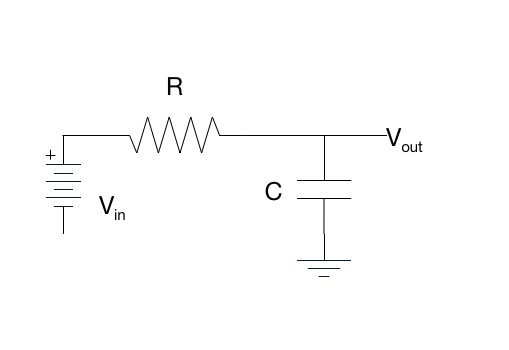
\includegraphics[scale=0.5]{lowpassFilter.jpg} \\
        Derivation of Low-Pass Transfer Function (RC): \\
        We have attained this from eq. (1.26) from the text: \\
        \begin{equation}
            X_C = \frac{1}{\omega*C}
        \end{equation}
        where $\omega$ is the frequency of the signal, $X_C$ is the reactance and $C$ is the capacitance.\\
        So treating the above diagram as a voltage divider and assuming there is no phase shift and neglecting inductance, we can make the following approximation by replacing the following in equation (4): $R_2$ with $C$, $R_1$ with $R$, and we generate the new approximate transfer equation...
        \begin{equation}
            \frac{V_{out}}{V_{in}} \approx \frac{X_C}{R + X_C}
        \end{equation}
        Substituting eq.(5) into (6): \\
        \begin{equation}
            \frac{V_{out}}{V_{in}} \approx \frac{\frac{1}{\omega*C}}{R+\frac{1}{\omega*C}}
        \end{equation}
        And multiplying the right side of (7) by $\omega*C$: \\
        \begin{equation}
            \frac{V_{out}}{V_{in}} \approx \frac{1}{1+\omega*R*C}
        \end{equation}
        As you can see, eq. (8) demonstrates that as your frequency $\omega$ increases, relative output voltage decreases, the transfer function approaches 1 at lower frequencies.
        
        \item A high-pass circuit contains a high-pass filter, which blocks low frequencies and allows high frequency signals to pass. It is similar to the low-pass circuit, but now, for RC circuits, the resistor is in the lower leg of the divider and the capacitor is in the upper leg of the divider, and for LR circuits, the inductor is in the lower leg while the resistor is in the upper leg.\\
        Example (only the RC circuit is pictured):\\
        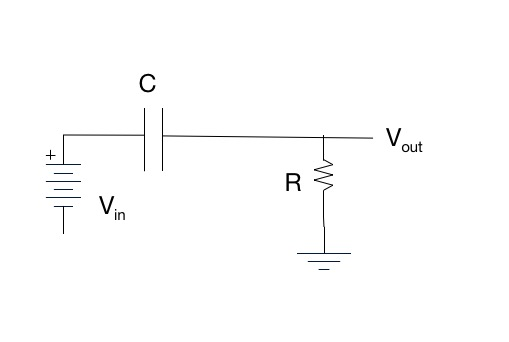
\includegraphics[scale=0.5]{highpass.jpg} \\
        Derivation of High-Pass Transfer Function (RC): \\
        Following a similar explanation to the derivation to the lower pass and using eq. (5), we can make the following approximation by replacing the following in equation (4): $R_1$ with $C$, $R_2$ with $R$, and we generate the new approximate transfer equation...
        \begin{equation}
            \frac{V_{out}}{V_{in}} \approx \frac{R}{R + X_C}
        \end{equation}
        Substituting eq.(5) into (9): \\
        \begin{equation}
            \frac{V_{out}}{V_{in}} \approx \frac{R}{R+\frac{1}{\omega*C}}
        \end{equation}
        And multiplying the right side of (10) by $\omega*C$: \\
        \begin{equation}
            \frac{V_{out}}{V_{in}} \approx \frac{\omega*R*C}{1+\omega*R*C}
        \end{equation}
        As you can see, eq. (11) demonstrates that as your frequency $\omega$ increases, a higher ratio of high frequency signals pass through.
        
        \item Note: A load can be added to each of these circuits...
    \end{enumerate}
\end{enumerate}
\end{document}